\documentclass{standalone}
\usepackage{tikz}
\usetikzlibrary{patterns, positioning}


\begin{document}
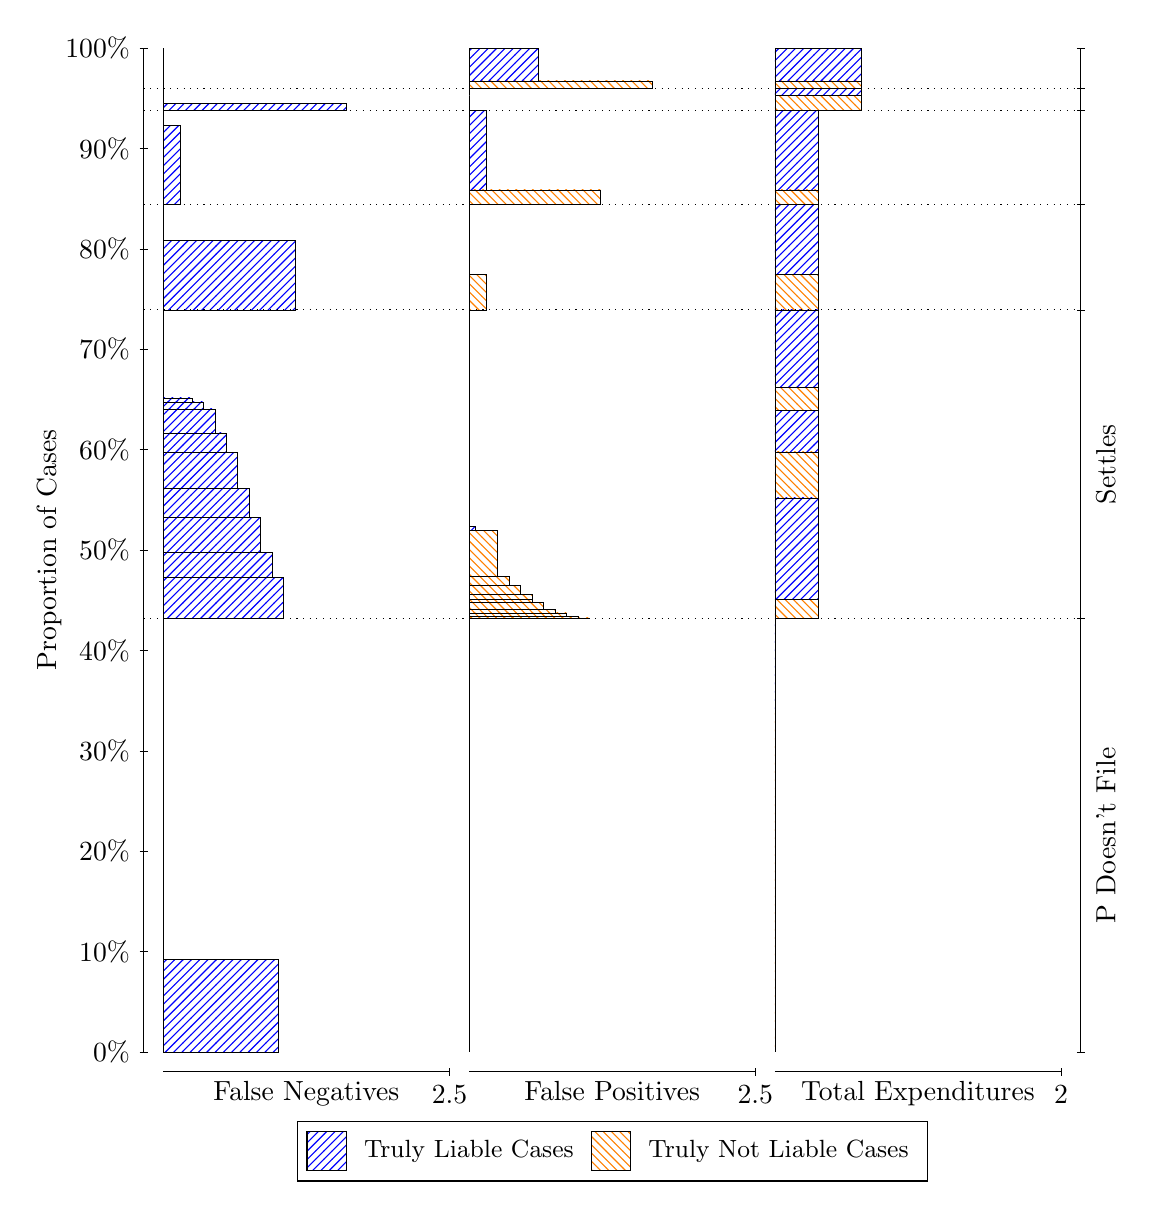
\begin{tikzpicture}
\draw[black, very thin] (1.5,1.75) -- (1.5,14.5);
\node[rotate=90, text=black, anchor=center] at (0.3, 8.125) {Proportion of Cases};
\draw[black, very thin] (1.45,1.75) -- (1.55,1.75);
\node[text=black, anchor=east] at (1.45, 1.75) {0\%};
\draw[black, very thin] (1.45,3.025) -- (1.55,3.025);
\node[text=black, anchor=east] at (1.45, 3.025) {10\%};
\draw[black, very thin] (1.45,4.3) -- (1.55,4.3);
\node[text=black, anchor=east] at (1.45, 4.3) {20\%};
\draw[black, very thin] (1.45,5.575) -- (1.55,5.575);
\node[text=black, anchor=east] at (1.45, 5.575) {30\%};
\draw[black, very thin] (1.45,6.85) -- (1.55,6.85);
\node[text=black, anchor=east] at (1.45, 6.85) {40\%};
\draw[black, very thin] (1.45,8.125) -- (1.55,8.125);
\node[text=black, anchor=east] at (1.45, 8.125) {50\%};
\draw[black, very thin] (1.45,9.4) -- (1.55,9.4);
\node[text=black, anchor=east] at (1.45, 9.4) {60\%};
\draw[black, very thin] (1.45,10.675) -- (1.55,10.675);
\node[text=black, anchor=east] at (1.45, 10.675) {70\%};
\draw[black, very thin] (1.45,11.95) -- (1.55,11.95);
\node[text=black, anchor=east] at (1.45, 11.95) {80\%};
\draw[black, very thin] (1.45,13.225) -- (1.55,13.225);
\node[text=black, anchor=east] at (1.45, 13.225) {90\%};
\draw[black, very thin] (1.45,14.5) -- (1.55,14.5);
\node[text=black, anchor=east] at (1.45, 14.5) {100\%};

\draw[black, very thin] (13.4,1.75) -- (13.4,14.5);
\draw[black, very thin] (13.35,1.75) -- (13.45,1.75);
\node[anchor=west] at (13.35, 1.75) {};
\draw[black, very thin] (13.35,7.2537) -- (13.45,7.2537);
\node[anchor=west] at (13.35, 7.2537) {};
\draw[black, very thin] (13.35,11.174) -- (13.45,11.174);
\node[anchor=west] at (13.35, 11.174) {};
\draw[black, very thin] (13.35,12.512) -- (13.45,12.512);
\node[anchor=west] at (13.35, 12.512) {};
\draw[black, very thin] (13.35,13.706) -- (13.45,13.706);
\node[anchor=west] at (13.35, 13.706) {};
\draw[black, very thin] (13.35,13.991) -- (13.45,13.991);
\node[anchor=west] at (13.35, 13.991) {};
\draw[black, very thin] (13.35,14.5) -- (13.45,14.5);
\node[anchor=west] at (13.35, 14.5) {};

\draw[black, very thin, pattern color=blue, pattern=north east lines] (1.75,1.75) rectangle (3.2033,2.9221);
\draw[black, very thin, pattern color=orange, pattern=north west lines] (1.75,2.9221) rectangle (1.75,7.2537);
\draw[black, very thin, pattern color=blue, pattern=north east lines] (1.75,7.2537) rectangle (3.276,7.7763);
\draw[black, very thin, pattern color=blue, pattern=north east lines] (1.75,7.7763) rectangle (3.1307,8.0946);
\draw[black, very thin, pattern color=blue, pattern=north east lines] (1.75,8.0946) rectangle (2.9853,8.5374);
\draw[black, very thin, pattern color=blue, pattern=north east lines] (1.75,8.5374) rectangle (2.84,8.9066);
\draw[black, very thin, pattern color=blue, pattern=north east lines] (1.75,8.9066) rectangle (2.6947,9.3675);
\draw[black, very thin, pattern color=blue, pattern=north east lines] (1.75,9.3675) rectangle (2.5493,9.6129);
\draw[black, very thin, pattern color=blue, pattern=north east lines] (1.75,9.6129) rectangle (2.404,9.916);
\draw[black, very thin, pattern color=blue, pattern=north east lines] (1.75,9.916) rectangle (2.2587,10.007);
\draw[black, very thin, pattern color=blue, pattern=north east lines] (1.75,10.007) rectangle (2.1133,10.057);
\draw[black, very thin, pattern color=orange, pattern=north west lines] (1.75,10.057) rectangle (1.75,11.174);
\draw[black, very thin, pattern color=blue, pattern=north east lines] (1.75,11.174) rectangle (3.4213,12.056);
\draw[black, very thin, pattern color=orange, pattern=north west lines] (1.75,12.056) rectangle (1.75,12.512);
\draw[black, very thin, pattern color=blue, pattern=north east lines] (1.75,12.512) rectangle (1.968,13.521);
\draw[black, very thin, pattern color=orange, pattern=north west lines] (1.75,13.521) rectangle (1.75,13.706);
\draw[black, very thin, pattern color=blue, pattern=north east lines] (1.75,13.706) rectangle (4.0753,13.798);
\draw[black, very thin, pattern color=orange, pattern=north west lines] (1.75,13.798) rectangle (1.75,13.991);
\draw[black, very thin, pattern color=orange, pattern=north west lines] (1.75,13.991) rectangle (1.75,14.084);
\draw[black, very thin, pattern color=blue, pattern=north east lines] (1.75,14.084) rectangle (1.75,14.5);
\draw[black, very thin, pattern color=orange, pattern=north west lines] (5.6333,1.75) rectangle (5.6333,6.0815);
\draw[black, very thin, pattern color=blue, pattern=north east lines] (5.6333,6.0815) rectangle (5.6333,7.2537);
\draw[black, very thin, pattern color=orange, pattern=north west lines] (5.6333,7.2537) rectangle (7.1593,7.2632);
\draw[black, very thin, pattern color=orange, pattern=north west lines] (5.6333,7.2632) rectangle (7.014,7.2795);
\draw[black, very thin, pattern color=orange, pattern=north west lines] (5.6333,7.2795) rectangle (6.8687,7.3252);
\draw[black, very thin, pattern color=orange, pattern=north west lines] (5.6333,7.3252) rectangle (6.7233,7.3664);
\draw[black, very thin, pattern color=orange, pattern=north west lines] (5.6333,7.3664) rectangle (6.578,7.4614);
\draw[black, very thin, pattern color=orange, pattern=north west lines] (5.6333,7.4614) rectangle (6.4327,7.4944);
\draw[black, very thin, pattern color=orange, pattern=north west lines] (5.6333,7.4944) rectangle (6.4327,7.5567);
\draw[black, very thin, pattern color=orange, pattern=north west lines] (5.6333,7.5567) rectangle (6.2873,7.6798);
\draw[black, very thin, pattern color=orange, pattern=north west lines] (5.6333,7.6798) rectangle (6.142,7.7875);
\draw[black, very thin, pattern color=orange, pattern=north west lines] (5.6333,7.7875) rectangle (5.9967,8.3709);
\draw[black, very thin, pattern color=blue, pattern=north east lines] (5.6333,8.3709) rectangle (5.706,8.4206);
\draw[black, very thin, pattern color=blue, pattern=north east lines] (5.6333,8.4206) rectangle (5.6333,11.174);
\draw[black, very thin, pattern color=orange, pattern=north west lines] (5.6333,11.174) rectangle (5.8513,11.63);
\draw[black, very thin, pattern color=blue, pattern=north east lines] (5.6333,11.63) rectangle (5.6333,12.512);
\draw[black, very thin, pattern color=orange, pattern=north west lines] (5.6333,12.512) rectangle (7.3047,12.697);
\draw[black, very thin, pattern color=blue, pattern=north east lines] (5.6333,12.697) rectangle (5.8513,13.706);
\draw[black, very thin, pattern color=orange, pattern=north west lines] (5.6333,13.706) rectangle (5.6333,13.898);
\draw[black, very thin, pattern color=blue, pattern=north east lines] (5.6333,13.898) rectangle (5.6333,13.991);
\draw[black, very thin, pattern color=orange, pattern=north west lines] (5.6333,13.991) rectangle (7.9587,14.084);
\draw[black, very thin, pattern color=blue, pattern=north east lines] (5.6333,14.084) rectangle (6.5053,14.5);
\draw[black, very thin, pattern color=orange, pattern=north west lines] (9.5167,1.75) rectangle (9.5167,6.0815);
\draw[black, very thin, pattern color=blue, pattern=north east lines] (9.5167,6.0815) rectangle (9.5167,7.2537);
\draw[black, very thin, pattern color=orange, pattern=north west lines] (9.5167,7.2537) rectangle (10.062,7.4944);
\draw[black, very thin, pattern color=blue, pattern=north east lines] (9.5167,7.4944) rectangle (10.062,8.7879);
\draw[black, very thin, pattern color=orange, pattern=north west lines] (9.5167,8.7879) rectangle (10.062,9.3712);
\draw[black, very thin, pattern color=blue, pattern=north east lines] (9.5167,9.3712) rectangle (10.062,9.8939);
\draw[black, very thin, pattern color=orange, pattern=north west lines] (9.5167,9.8939) rectangle (10.062,10.187);
\draw[black, very thin, pattern color=blue, pattern=north east lines] (9.5167,10.187) rectangle (10.062,11.174);
\draw[black, very thin, pattern color=orange, pattern=north west lines] (9.5167,11.174) rectangle (10.062,11.63);
\draw[black, very thin, pattern color=blue, pattern=north east lines] (9.5167,11.63) rectangle (10.062,12.512);
\draw[black, very thin, pattern color=orange, pattern=north west lines] (9.5167,12.512) rectangle (10.062,12.697);
\draw[black, very thin, pattern color=blue, pattern=north east lines] (9.5167,12.697) rectangle (10.062,13.706);
\draw[black, very thin, pattern color=orange, pattern=north west lines] (9.5167,13.706) rectangle (10.607,13.898);
\draw[black, very thin, pattern color=blue, pattern=north east lines] (9.5167,13.898) rectangle (10.607,13.991);
\draw[black, very thin, pattern color=orange, pattern=north west lines] (9.5167,13.991) rectangle (10.607,14.084);
\draw[black, very thin, pattern color=blue, pattern=north east lines] (9.5167,14.084) rectangle (10.607,14.5);
\draw[black, dotted] (1.5,7.2537) -- (13.4,7.2537);
\draw[black, dotted] (1.5,11.174) -- (13.4,11.174);
\draw[black, dotted] (1.5,12.512) -- (13.4,12.512);
\draw[black, dotted] (1.5,13.706) -- (13.4,13.706);
\draw[black, dotted] (1.5,13.991) -- (13.4,13.991);
\draw[black, very thin] (1.75,1.5) -- (5.3833,1.5);
\node[text=black, anchor=north] at (3.5667, 1.5) {False Negatives};
\draw[black, very thin] (5.3833,1.45) -- (5.3833,1.55);
\node[text=black, anchor=north] at (5.3833, 1.45) {2.5};

\draw[black, very thin] (5.6333,1.5) -- (9.2667,1.5);
\node[text=black, anchor=north] at (7.45, 1.5) {False Positives};
\draw[black, very thin] (9.2667,1.45) -- (9.2667,1.55);
\node[text=black, anchor=north] at (9.2667, 1.45) {2.5};

\draw[black, very thin] (9.5167,1.5) -- (13.15,1.5);
\node[text=black, anchor=north] at (11.333, 1.5) {Total Expenditures};
\draw[black, very thin] (13.15,1.45) -- (13.15,1.55);
\node[text=black, anchor=north] at (13.15, 1.45) {2};

\node[text=black, centered, rotate=90] at (13.72, 4.5018) {P Doesn't File};
\node[text=black, centered, rotate=90] at (13.72, 9.2139) {Settles};





\draw (7.449999999999999,1.5) node[draw=none] (baseCoordinate) {};
\begin{scope}[align=center]
        \matrix[scale=0.5, draw=black, below=0.5cm of baseCoordinate, nodes={draw}, column sep=0.1cm]{
            \node[rectangle, draw, minimum width=0.5cm, minimum height=0.5cm, pattern color=blue, pattern=north east lines] {}; &
            \node[draw=none, font=\small, text=black] (B) {Truly Liable Cases}; &
            \node[rectangle, draw, minimum width=0.5cm, minimum height=0.5cm, pattern color=orange, pattern=north west lines] {}; &
            \node[draw=none, font=\small, text=black] (B) {Truly Not Liable Cases}; \\
            };
\end{scope}

\end{tikzpicture}
\end{document}